% Giacomo Petrillo
% lezione di Punzi

\section{Limite centrale}

Consideriamo la media aritmetica di $n$ variabili identiche:
\begin{equation*}
	\bar x \is \frac1n \sum_{i=1}^n x_i.
\end{equation*}
Se la media e la varianza delle $x_i$ sono $\mu$ e $\sigma^2$,
dalle proprietà del valore atteso si ricava immediatamente che
\begin{equation*}
	E[\bar x] = \mu, \quad \var[\bar x] = \frac{\sigma^2}{n}.
\end{equation*}
Definiamo
\begin{equation*}
	y_n \is \frac{\bar x - \mu}{\sigma / \sqrt n},
\end{equation*}
che ha media~0 e varianza~1.
Dalle proprietà della funzione caratteristica si ricava che
\begin{equation*}
	\phi_{y_n}(t) = e^{-\frac{it\mu}{\sigma}\sqrt n} \phi_x\left(\frac t\sigma \frac1{\sqrt n}\right)^n,
\end{equation*}
dove $\phi_x$ è la funzione caratteristica delle $x_i$. Prendiamone il logaritmo:
\begin{equation*}
	\log\phi_{y_n}(t) = -\frac{it\mu}{\sigma}\sqrt n + n\log\phi_x\left(\frac t\sigma \frac1{\sqrt n}\right).
\end{equation*}
Dagli sviluppi del logaritmo e della funzione caratteristica
\begin{align*}
	\log(1+u) &= u - \frac12 u^2 + \dotsb \\
	\phi_x(u) &= \phi_x(0) + \phi_x'(0)u + \frac12 \phi_x''(0) u^2 + \dotsb
\end{align*}
e usando i momenti
\begin{align*}
	\phi_x(0) &= 1 \\
	\mu = i^{-1}\phi_x'(0) \rightarrow \phi_x'(0) &= i\mu \\
	\sigma^2 = i^{-2}\phi_x''(0) - \mu^2 \rightarrow \phi_x''(0) &= -(\mu^2+\sigma^2)
\end{align*}
otteniamo che
\begin{align*}
	\log\phi_{y_n}(t)
	&= -\frac{it\mu}{\sigma}\sqrt n + {} \\
	&\phantom{{}={}} + n \log\left(1 + \phi_x'(0) \frac t\sigma \frac1{\sqrt n}
	+ \frac12 \phi_x''(0) \frac{t^2}{\sigma^2} \frac1n
	+ O\left(\frac1{n\sqrt n}\right) \right) = \\
	&= -\frac{it\mu}{\sigma}\sqrt n
	+ n \left( \phi_x'(0) \frac t\sigma \frac1{\sqrt n}
	+ \frac12 \phi_x''(0) \frac{t^2}{\sigma^2} \frac 1n + {}\right. \\
	&\left.\phantom{= -\frac{it\mu}{\sigma}\sqrt n + n\left(\vphantom{\frac1{\sqrt n}}\right.}
	- \frac12 \phi_x'(0)^2 \frac{t^2}{\sigma^2} \frac 1n 
	+ O\left(\frac1{n\sqrt n}\right) \right) = \\
	&= -\frac{it\mu}{\sigma}\sqrt n
	+ \frac{it\mu}{\sigma}\sqrt n
	+ \frac12 (-\mu^2 - \sigma^2 + \mu^2) \frac{t^2}{\sigma^2} + O\left(\frac1{\sqrt n}\right) = \\
	&= -\frac{t^2}2 + O\left(\frac1{\sqrt n}\right),
\end{align*}
quindi abbiamo il limite
\begin{equation*}
	\phi_{y_\infty}(t) = e^{-t^2/2}.
\end{equation*}
Ricaviamo la pdf con la trasformata inversa:
\marginpar{Andrebbe chiarito il passaggio dal limite sulle caratteristiche a quello sulle pdf.
Usare il \autoref{th:paullevy}.}
\begin{align*}
	p(y)
	&= \frac1{2\pi} \int_{-\infty}^\infty \de t\, e^{-ity} e^{-t^2/2} = \\
	&= \frac1{2\pi} \int_{-\infty}^\infty \de t\,
	\exp\left( -\left(\frac t{\sqrt 2} + \frac{iy}{\sqrt 2}\right)^2 - \frac{y^2}2 \right) = \\
	&= \frac1{2\pi} \sqrt{2\pi} e^{-y^2/2} = \\
	&= \frac1{\sqrt{2\pi}} e^{-y^2/2};
\end{align*}
questa distribuzione si chiama \emph{gaussiana} (o \emph{normale}).
Abbiamo quindi dimostrato il
\begin{theorem}[del limite centrale]
	\label{th:limitecentrale}
	Sia $x$ variabile che ammette media e varianza e con funzione caratteristica sviluppabile in serie di potenze su $\R$,
	allora la somma di $n$ variabili indipendenti identiche a $x$ normalizzata in modo da avere media nulla e varianza unitaria ha distribuzione gaussiana nel limite $n\to\infty$.
\end{theorem}
Questa è una forma debole del teorema del limite centrale, che sotto opportune ipotesi vale anche sommando variabili con distribuzioni diverse.

\chapter{Inferenza}

L'inferenza cerca di risolvere il problema:
<<ho delle misure che voglio descrivere con la probabilità,
qual è la distribuzione che devo usare, ovvero \emph{assegnare alle misure}?>>
Affinché la questione sia ben posta bisogna fissare un'insieme di distribuzioni, il \emph{modello},
tra cui in qualche modo scegliere quelle che descrivono meglio le misure.
Tipicamente descriverò una famiglia di distribuzioni al variare di parametri reali,
ad esempio se <<scelgo un modello poissoniano>> di solito intendo la famiglia di distribuzioni
\begin{equation*}
	P(k) = \frac{\mu^k}{k!}e^{-\mu}
\end{equation*}
in cui il parametro è $\mu$.
Il punto diventa allora dire quali siano i valori di $\mu$ ``giusti'' e in che senso siano ``giusti''.

\begin{definition}[Modello]
	Un \emph{modello} è una famiglia di distribuzioni di probabilità sulla stessa variabile.
	Una \emph{parametrizzazione} del modello è una funzione iniettiva
	\marginpar{Nell'interpretazione bayesiana $p(x;\theta)=p(x|\theta)$
	la richiesta di iniettività cade.}
	da uno \emph{spazio del parametro} $\Theta$
	al modello.
	L'argomento della parametrizzazione si chiama \emph{parametro}.
	Detta $x$ la variabile e $\theta$ il parametro,
	gli elementi del modello, valutati in $x$, si indicano con $p(x;\theta)$.
\end{definition}

\section{Likelihood}

\begin{definition}[Likelihood]
	Dato un modello per $x$ parametrizzato da $\theta$
	e fissato un valore $x_0$ della variabile,
	la \emph{likelihood} (o \emph{verosimiglianza}) è la funzione di $\theta$
	che restituisce la distribuzione $\theta$ valutata in $x_0$:
	\begin{equation*}
		\mathcal L(\theta) \is p(x_0;\theta).
	\end{equation*}
\end{definition}

Il senso di definire la likelihood
è che in un esperimento il valore fissato della variabile è quello misurato.

Notiamo che la likelihood non è in generale una distribuzione per $\theta$.
Spesso ci interessa il caso di misure ripetute di una stessa quantità e di come vari l'inferenza all'aumentare del numero di misure, in questo caso la likelihood si scrive
\begin{equation*}
	\mathcal L(\theta) = p(x_1;\theta) p(x_2;\theta) \dotsm p(x_N;\theta).
\end{equation*}

\begin{example}
	\begin{figure}
		\centering
		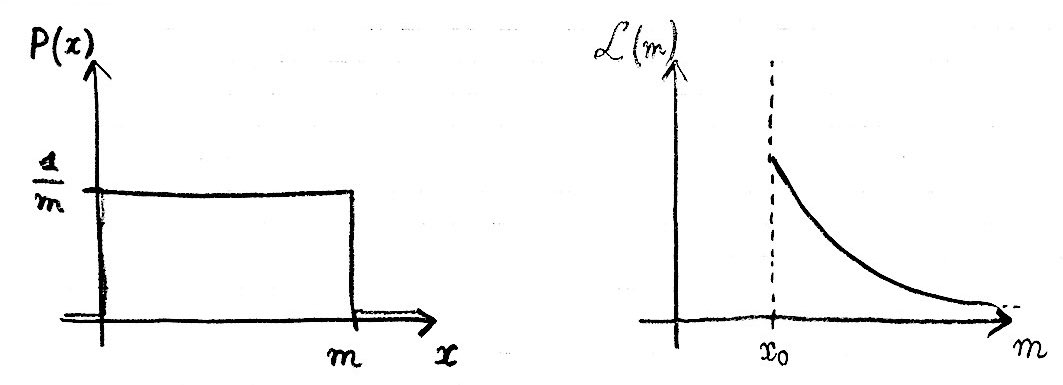
\includegraphics[width=9cm]{likelihood_uniforme}
		\caption{\label{fig:likeunif}%
		Distribuzione uniforme e likelihood.}
	\end{figure}
	Consideriamo una pdf uniforme
	\begin{equation*}
		p(x;m)
		= \frac1m \chi_{(0,m)}(x)
		= \begin{cases}
			\frac 1m & 0<x<m \\
			0 & \text{altrimenti.}
		\end{cases}
	\end{equation*}
	Fissata una misura $x_0$ la likelihood è (vedi \autoref{fig:likeunif})
	\begin{equation*}
		\mathcal L(m)
		= \frac1m \chi_{(x_0,\infty)}(m)
		= \begin{cases}
			\frac 1m & m > x_0 \\
			0 & 0 < m \le x_0.
		\end{cases}
	\end{equation*}
\end{example}

Se cambiamo variabile, la likelihood trasforma con una costante:
\begin{align*}
	y &= f(x) \\
	p(y;\theta) &= \frac{p(x;\theta)}{|f'(x)|} \\
	\mathcal L_y(\theta) &= \frac{\mathcal L_x(\theta)}{|f'(x_0)|}.
\end{align*}
quindi diciamo che la likelihood è definita a meno di una costante moltiplicativa positiva.
Se invece cambiamo parametro, la likelihood trasforma in modo banale:
\begin{align*}
	\eta &= g(\theta) \\
	\mathcal L_\eta(\eta) &= \mathcal L_\theta(g^{-1}(\eta)).
\end{align*}
Se combino misure indipendenti, le likelihood si moltiplicano:
\begin{align*}
	p(x,y;\theta) &= p(x;\theta) p(y;\theta) \\
	\rightarrow \mathcal L_{x,y}(\theta) &= \mathcal L_x(\theta) \mathcal L_y(\theta).
\end{align*}

\section{Inferenza bayesiana}

Supponiamo di considerare il parametro come una variabile aleatoria.
Allora possiamo porre
\begin{equation*}
	p(x|\theta) = p(x;\theta)
\end{equation*}
e applicare il teorema di Bayes per ricavare $p(\theta|x)$:
\begin{equation*}
	p(\theta|x) = \frac{p(x|\theta)p(\theta)}{p(x)}
\end{equation*}
che, fissata una misura $x_0$, diventa
\begin{equation*}
	p(\theta|x_0) = \frac{\mathcal L(\theta) p(\theta)}{p(x_0)}.
\end{equation*}
Si chiamano $p(\theta|x_0)$ \emph{posteriore} e $p(\theta)$ \emph{priore}.
Il termine $p(x_0)$ è un fattore di normalizzazione, in effetti
\begin{equation*}
	p(x_0) = \int \de \theta\, \mathcal L(\theta) p(\theta).
\end{equation*}
Il termine interessante è il priore, perché richiede in pratica di scegliere un'ulteriore distribuzione oltre al modello.
Se abbiamo il priore, l'inferenza è finita, perché tutto quello che la teoria della probabilità ci può dire su $\theta$ in seguito alla misura è racchiuso in $p(\theta|x_0)$.

% qui c'era una parte sulle sistematiche,
% l'ho spostata all'inizio del 13 ottobre

Secondo l'interpretazione frequentista della probabilità,
per assegnare un priore a $\theta$ è richiesto che sia quantomeno possibile una verifica empirica della distribuzione di $\theta$.
Tuttavia questo restringe molto i casi in cui possiamo ricavare il posteriore.
Nell'interpretazione bayesiana una distribuzione di probabilità rappresenta la conoscenza soggettiva che abbiamo di una quantità.
Allora possiamo scegliere ad arbitrio il priore.
Se questa scelta arbitraria sembra un problema fondamentale,
ricordiamo al lettore che in definitiva anche il modello è arbitrario.
Si vede subito che non esiste un priore privilegiato perché cambiando parametro il priore trasforma in modo non banale, a differenza della likelihood.

